\documentclass[12pt]{article}
\usepackage[margin=1in]{geometry} 
\usepackage{amsmath,amsthm,amssymb,amsfonts}
\usepackage{enumitem}
\usepackage{tabu}
\usepackage{xcolor}
\usepackage{mathtools}
\usepackage{tcolorbox} 
\usepackage{changepage} 
\usepackage{kpfonts}
\usepackage{picture}
\usepackage{venndiagram}
\usepackage{graphicx}

\newcommand{\prob}[1]{\mathbb{P}(#1)}
\newcommand{\condprob}[2]{\mathbb{P}(#1 \text{ } \lvert \text{ } #2)}

\newcommand{\N}{\mathbb{N}}
\newcommand{\Z}{\mathbb{Z}}
\newcommand{\R}{\mathbb{R}}
\newcommand{\field}{\mathcal{F}}

\begin{document}
% ================================================================================================================================
% ================================================================================================================================
\section*{CHAPTER 1}

\subsection*{Conjuction Fallacy}
\noindent
The probability of the joint realization of two events, say $A$ and $B$, cannot be larger than the probability of either of the two events, considered on its own. Denoting the probabilities of the events by $\mathbb{P}(A)$, $\mathbb{P}(B)$, and $\mathbb{P}(A \cap B)$, the basic law of probability law takes the form,

\begin{align*}
\mathbb{P}(A \cap B) \leq \mathbb{P}(A) \enspace \text{  or  } \enspace \mathbb{P}(A \cap B) \mathbb{P}(B).
\end{align*}

\subsection*{Binary Relations}
\noindent
\textbf{Definition} A \textit{Binary Relation}, given sets $X$ and $Y$, is a set $R$ such that

\begin{equation*}
R \subseteq X \times Y.
\end{equation*}

\noindent
A binary relation is a set of ordered pairs $xy \in X \times Y$, where $xy$ is an abbreviation for $(x,y)$. If $X=Y$, then $R$ is said to be a binary relation on $X$. A binary relations $R$ is a \textit{quasi order} on a set $X$ if it is \textit{reflexive} and \textit{transitive}. That is, for all $x$, $y$, and $z$ in $X$, 

\begin{align*}
xRx && (\text{reflexivity}) \\
xRy \text{ } \& \text{ } yRz \implies xRz && (\text{reflexivity})
\end{align*}

\noindent
A binary relation $R$ is an \textit{equivalence relation} on a set $X$ if it is \textit{reflexive}, \textit{transitive}, and \textit{symmetric} on $X$. for all $x$, $y$, and $z$ in $X$,

\begin{equation*}
xRy \iff yRx.
\end{equation*}

\subsection*{Partitions}
\noindent
The family $\mathcal{X} = \big \{ [x] \lvert x \in X \big \}$ of subsets is called a \textit{partition} of $X$ induced by $\sim$. Any partition $\mathcal{X}$ of $X$ satisfies the following three properties,

\begin{enumerate}
\item $Y \in X$ implies $Y \neq \emptyset$;
\item $Y,Z \in \mathcal{X}$ and $Y \neq Z$ imply $Y \cap Z \neq \emptyset$;
\item $\cup \mathcal{X} = X$.
\end{enumerate}

\noindent
Conversely, any family $\mathcal{X}$ of subsets of a set $X$ satisfying $[1]$, $[2]$, and $[3]$ is called a partition of $X$.

% ================================================================================================================================
% ================================================================================================================================
\section*{CHAPTER 2: Sample Spaces}

\subsection*{The Sample Space}
\noindent
What is critical is that all feasible outcomes have a description in the sample space. It is of no importance that the sample space contains outcomes that never happen in practice: in the framework of a probabilistic model, such outcomes may be assigned zero probability. \\

\noindent
A sample space which is either \textbf{finite} or \textbf{countable} is called \textit{discrete}.  \\

\begin{tcolorbox}
\begin{center}
Finite vs. Countable
\end{center}

\textbf{Finite}: A definite number. Not infinite. In other words it could be measured, or given a value.

\vspace*{.5cm}

\textbf{Countable}: Either finite or a countably infinite (implying that the cardinality of a countable set is a subset of $\N$). Elements of a countable set can always be counted one at a time and, although the counting may never finish, every element of the set is associated with a unique natural number.
\end{tcolorbox}

\subsection*{Concept of an Event}
\noindent
Fundamentally, an \textit{Event} is a subset of the sample space. In general, each event pertaining to a particular experiment may be identified with a subset of the relevant sample space. However, with respect to the converse, the general assumption that all subsets of the sample space are events to which a probability could be assigned would create mathematical difficulties.

\subsection*{Indicator Functions}
\noindent
\textbf{Definition}: An \textit{Indicator Function} is a function defined on a set $\Omega$ that indicates membership of an element in a subset of $X$ of $\Omega$. Let $\Omega$ be a non-empty set and $X$ a subset of $\Omega$. The indicator function on $X$ is a function $I_x : \Omega \rightarrow \{ 0,1 \}$ by,

\begin{equation*}
I_x(w) =  \begin{cases} 
      0 & w \in X \\
      1 & w \in \overline{X} \text{  } (\text{or } w \not \in X)
   \end{cases}
\end{equation*}

\noindent
Properties of Indicator Functions:

\begin{itemize}
\item For subsets $X, Y$ of $\Omega$, $I_{X \cap Y}=I_X \cdot I_Y$, i.e. for every $w \in \Omega$, $I_{X \cap Y}(w)=I_X(w) \cdot I_Y(w)$.
\item $I_{X \cup Y}=I_X + I_Y - I_{X \cap Y}$ (if $X,Y$ are disjoint, $I_{X \cup Y}=I_X + I_Y$)
\item $I_{A^C}=1-I_A$
\item If $X \subseteq Y$, then $I_X \subseteq I_Y$, i.e. $I_X(w) \leq I_Y(w)$ for every $w \in \Omega$.
\end{itemize}

% ================================================================================================================================
% ================================================================================================================================
\section*{CHAPTER 3: Probability and Area}

\subsection*{Axioms for a Field}
\noindent
\textbf{Definition}: Let $\Omega$ be a set. Let $\field$ be a nonempty collection of subsets of $\Omega$ satisfying the axioms

\begin{adjustwidth}{2.5em}{0pt}
\textbf{[F1]} For all $A, B \in \field$, $A \cup B \in \field$.

\vspace{.1cm}
\noindent
\textbf{[F2]} For each $A \in \field$, $\overline{A} \in \field$ also.
\end{adjustwidth}

\vspace{.5cm}
\noindent
\textbf{Theorem 3.2:} Let $\field$ be a field of subsets of $\Omega$. Then, 
\begin{frame}{}
\begin{enumerate}[label=(\roman*)]
\item $\Omega \in \field$
\item $\emptyset \in \field$
\item For all $A, B \in \field$, $A \setminus B = A \overline{B} \in \field$
\item $\bigcup\limits_{i=1}^{n} A_i \in \field$
\item $\bigcap\limits_{i=1}^{n} A_i \in \field$
 \makebox(0,0){\put(3,5\normalbaselineskip){%
               $\left.\rule{0pt}{2.2\normalbaselineskip}\right\}$ $\field$ is closed under finite union \textbf{and} finite intersection}}
\end{enumerate}
\end{frame}

\subsection*{Infinite Sample Spaces and $\sigma$-Fields}
\noindent
\textbf{Definition}: A field $(\Omega, \field)$ is called a $\sigma$-field if it is \textit{closed under countable union}, that is, if for any countable collection $A_1, \ldots, A_n, \ldots$ of sets in $\field$, we have $\bigcup_{n=1}^{\infty} A_n \in \field$. Note that for any sets $A_1, \ldots, A_n, \ldots$, we have

\begin{equation*}
\bigcap_{n=1}^{\infty} A_n = \overline{\bigcup_{n=1}^{\infty} \overline{A_n}}
\end{equation*}

\noindent
As a $\sigma$-field, $\field$ is closed under both countable union and complementation. We conclude that $\field$ is also closed under countable intersection.

\subsection*{Borel Fields}
\noindent
Recall that a set $S$ of real numbers is an \textit{open} set of $\R$ if for any $x \in S$, there exists some $\delta > 0$ such that whenever $\lvert x - y \rvert < \delta$, then $y \in S$. The standard family of events for $\R$ is a distinguished $\sigma$-field $\mathcal{B}$ containing all the open sets of $\R$. In fact, $\mathcal{B}$ is the `smallest' $\sigma$-field containing these open sets. The collection $\mathcal{B}$ is called the \textit{Borel Field} of $\R$, and the events in $\mathcal{B}$ are referred to as the \textit{Borel sets} of $\R$. These definitions extend naturally to the case where all the sample space is $\R^n$. 

\begin{center}
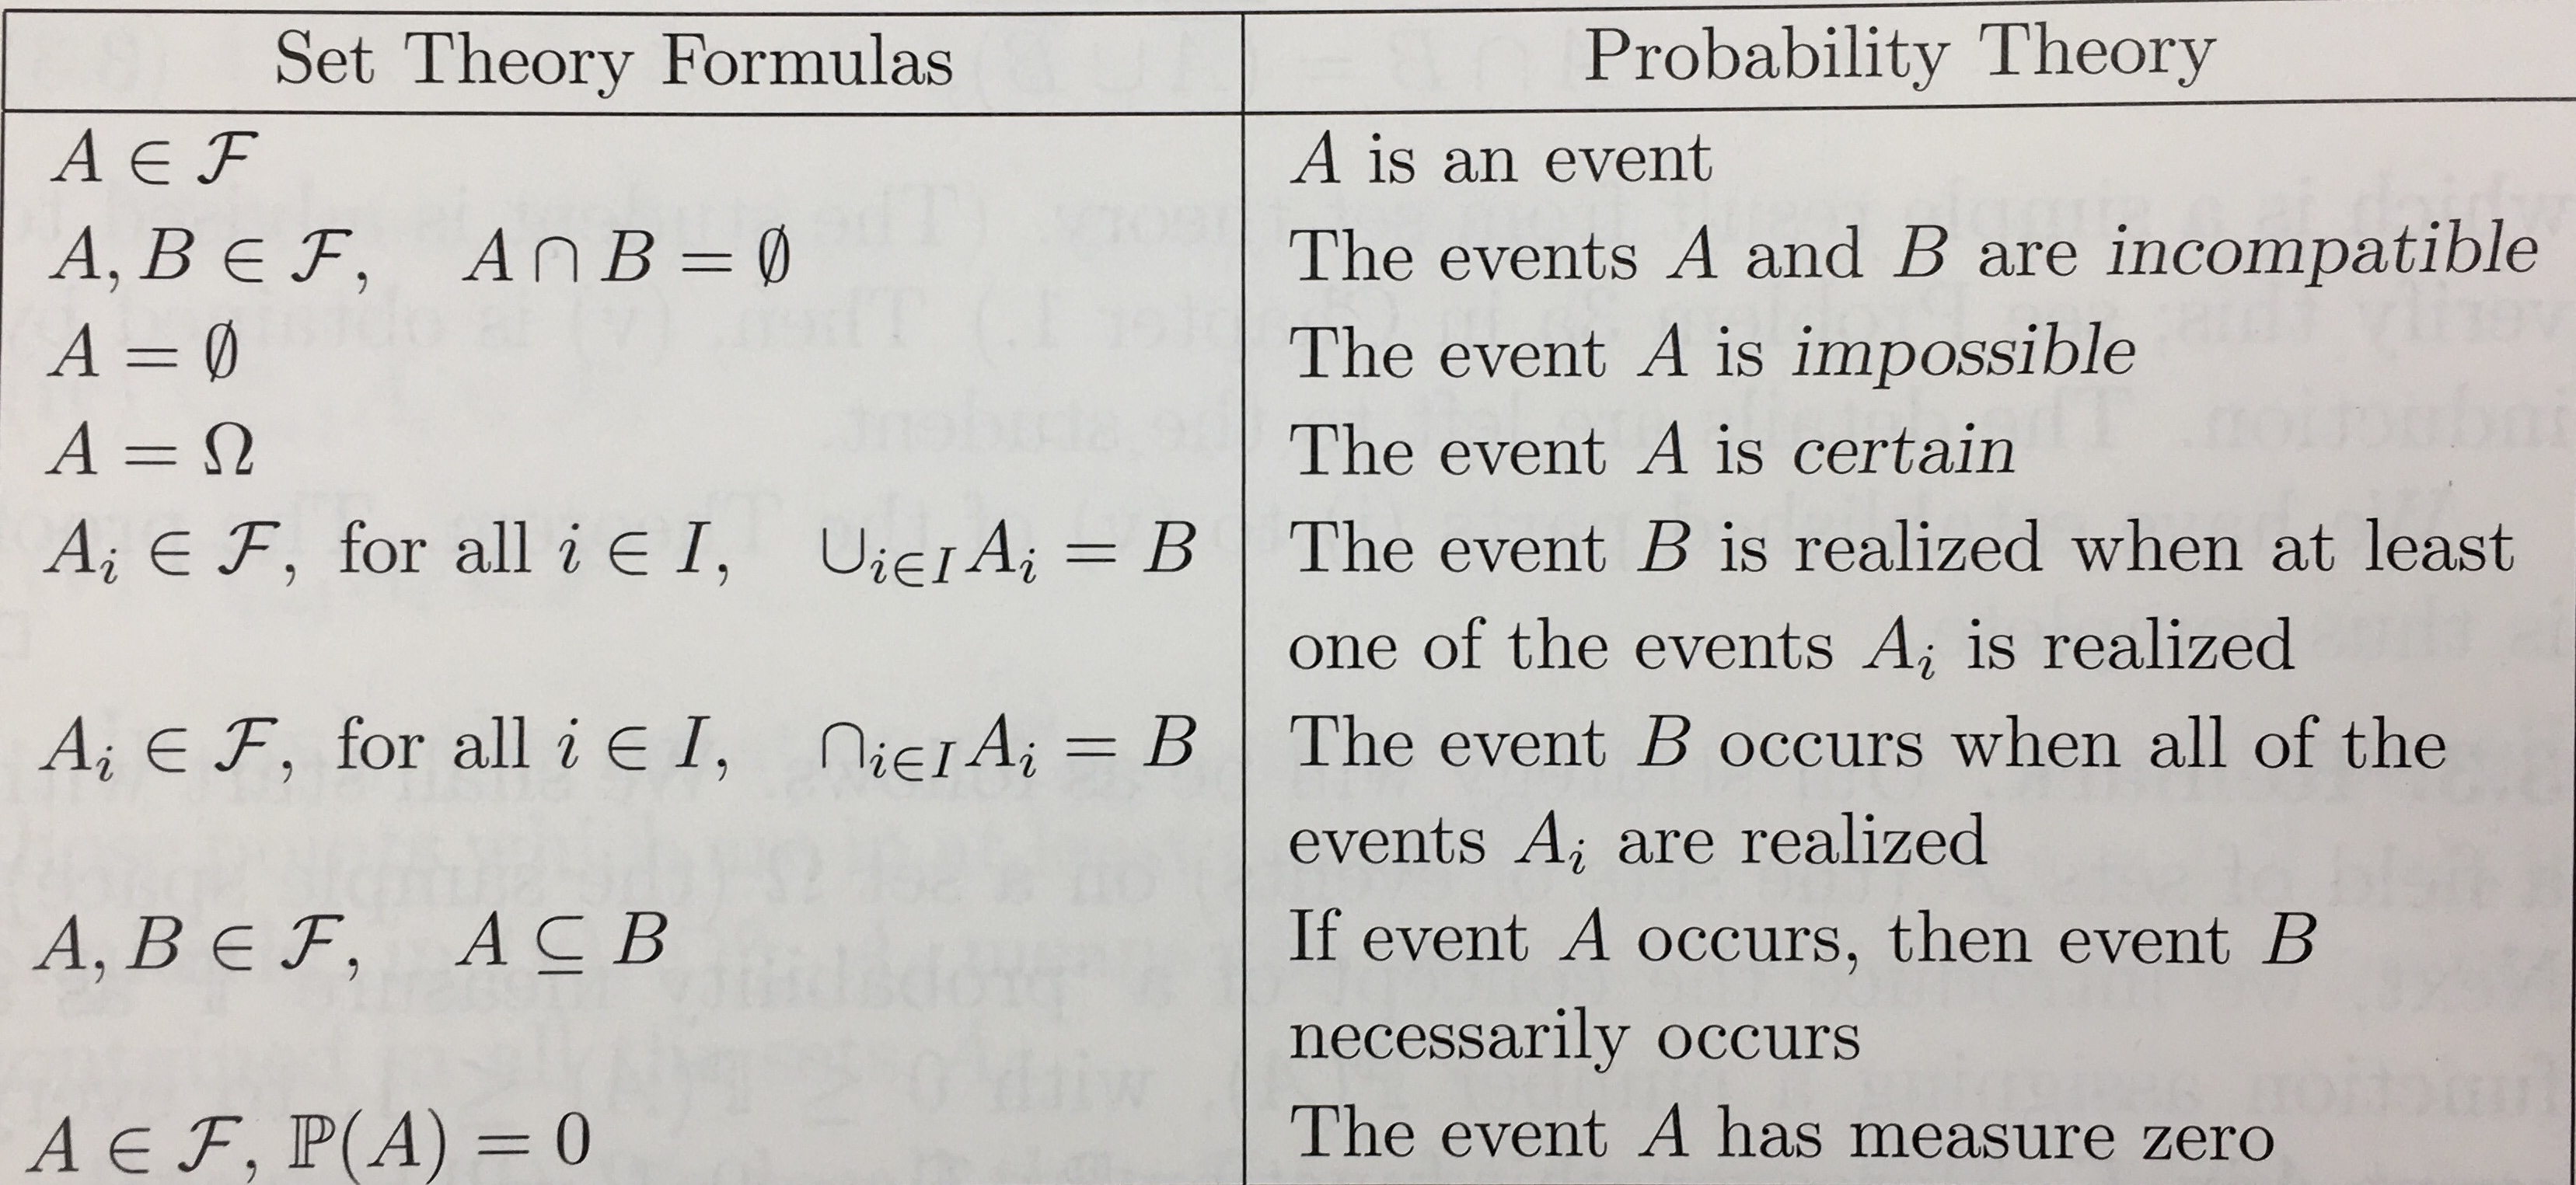
\includegraphics[width=9cm, height=5cm]{probthoerycommonterms}
\end{center}

\noindent
\subsection*{General Strategy}
We start with a field of sets $\field$ on a set $\Omega$. Then, we introduce the concept of a probability measure $\mathbb{P}$ as a function assigning a number $\mathbb{P}(A)$, with $0 \leq \mathbb{P}(A) \leq 1$, to every event $A$ in $\field$. This function $\mathbb{P} : \field \rightarrow [0,1]$ will be assumed to satisfy a number of axioms (given in Ch. 4). The probability measure $\mathbb{P}$ is not assumed in general to be defined on all subsets of the sample space due to the case of an uncountable sample space leading to a contradiction.

% ================================================================================================================================
% ================================================================================================================================
\section*{CHAPTER 4: Probability Measures}
We shall define a probability measure $\mathbb{P}$ as a function assigning a number $\mathbb{P}(A)$ to each event in $A$ in a field $\field$. For all events $A$, $\mathbb{P}$ will satisfy the following conditions,

\begin{enumerate}[label=(\roman*)]
\item $\mathbb{P}(\Omega) = 1$;
\item $0 \leq \mathbb{P}(A) \leq 1$;
\item $\mathbb{P}(A \cup B) = \mathbb{P}(A) + \mathbb{P}(B)$ for incompatible events $A,B$;
\item $\mathbb{P}(\bigcup_{i=1}^{n}) = \sum_{i=1}^{n} \mathbb{P}(A_i)$ for pairwise incompatible events $A_1, \ldots, A_n$ (\textit{finite additivity});
\end{enumerate}

\noindent
By requiring that if $A_1, \ldots, A_i, \ldots$ is a countably infinite sequence of pairwise incompatible events, then $\bigcup_{i=1}^{n} A_i$ is an event. Moreover, 

\begin{equation}
\mathbb{P} \big ( \bigcup_{i=1}^{\infty} \big ) = \sum_{i=1}^{\infty} \mathbb{P}(A_i).
\end{equation}

\subsection*{Finitely Additive Probability Space}
Let $\field$ be a field of sets on $\Omega$. Then, the triple $(\Omega, \field, \mathbb{P})$ is a \textit{finitely additive probability space} iff $\mathbb{P}$ is a real valued function on $\field$ satisfying the following three conditions: For all $A,B \in \field$,

\begin{itemize}
\item $[K1] \mathbb{P}(\Omega) = 1$;
\item $[K2] \mathbb{P}(A) \geq 0$;
\item $[K3]$ if $A \cap B = 0$, then $\mathbb{P}(A \cup B) = \mathbb{P}(A) + \mathbb{P}(B)$;
\end{itemize}

\noindent
The function $\mathbb{P}$ is called a \textit{probability measure}. In the special case where $\field$ is a $\sigma$-field, 

\begin{equation}
\mathbb{P} \big ( \bigcup_{i=1}^{\infty} \big ) = \sum_{i=1}^{\infty} \mathbb{P}(A_i)
\end{equation}

\noindent
holds for any countable family $\big \{ A_i \lvert i \in \N \big \}$ of pairwise disjoint events, then $(\Omega, \field, \mathbb{P})$ is called a \textit{probability space}. \\

\subsection*{Probability and Counting Measure}
\noindent
Suppose that $\Omega$ is a finite set, and let $\field$ be a field of its subsets. For any event $A \in \field$, we define

\begin{equation*}
\prob{A} = \frac{\lvert A \rvert}{\lvert \Omega \rvert}
\end{equation*}

\noindent
The value of the probability measure on $\mathbb{P}$ for a particular event $A$ is the ratio of the number of elements of $A$ to the total number of elements in the sample space $\Omega$. The probability measure is sometimes called the \textit{counting measure} and is appropriate when it makes sense to attribute an equal weight or likelihood to each point of the sample space.
\subsection*{Probability Distribution}

\noindent
\textbf{Definition}: Let $\Omega$ be a finite or countable sample space. Then $p$ is a \textit{probability distribution} on $\Omega$ iff $p$ is a real valued function on $\Omega$ satisfying

\begin{align*}
p(x) \geq 0 \text{ for all } x \in \Omega; \\
\sum_{x \in \Omega} p(x) = 1.
\end{align*}

\noindent
\textbf{Theorem}: Let $\field$ be a field of sets on a finite or countable sample space $\Omega$, and let $p$ be a probability distribution on $\Omega$. Define a function $\mathbb{P}$ on $\field$ by

\begin{equation}
\mathbb{P}(A) = \sum_{x \in A} p(x),
\end{equation}

\noindent
for all $A \in \field$. Then $(\Omega, \field, \mathbb{P})$ is a \textit{probability space}. When $(A_i)_{i \in I}$ is a sequence of pairwise events, with the index set $I$ being finite or countable, and each of the events $A_i$ being finite or countable, 

\begin{align*}
\sum_{i \in I} \mathbb{P}(A_i) & = \sum_{i \in I} \sum_{x \in A_i} p(x) \\
& = \sum_{x \in \bigcup_{i \in I} A_i} p(x) \\
& = \mathbb{P}(\bigcup_{i \in I} A_i)
\end{align*}

\subsection*{Remarks}
\noindent
The material in this chapter suggests that the notions of a field of events and of a probability measure are only considered with finite or countable sample spaces because the probability of any subset of the sample space could be computed from the probability distribution. With uncountable sample spaces, the notion of a probability distribution is useless. It turns out that `probability density functions' is a conceptual notion related to that of probability distributions.

% ================================================================================================================================
% ================================================================================================================================
\section*{CHAPTER 5: Basic Rules of Probability Calculus}
\noindent
\textbf{Theorem}: Let $\Omega$ be a sample space, and $(\Omega, \field, \mathbb{P})$ a finite additive probability space. We do note assume that $\Omega$ or $\field$ are finite. Then, for any events $A,B,C \in \field$,

\begin{enumerate}[label=(\roman*)]
\item $\prob{A} + \prob{\overline{A}} = 1$
\item $\prob{\emptyset}=0$
\item If $A_1, \ldots, A_n$ are incompatible events in $\field$, then

\begin{equation*}
\mathbb{P} \Big ( \sum_{j=1}^{n} A_j \Big ) = \sum_{j=1}^{n} \prob{A_j}
\end{equation*}

\item If $A \subseteq B$, then $\prob{A} \leq \prob{B}$
\item $\prob{A \cup  B} = \prob{A} + \prob{B} - \prob{A \cap B}$
\item 

\begin{align*}
\prob{A \cup B \cup C} =  \enspace & \prob{A} + \prob{B} + \prob{C} \\
& - \prob{AB} - \prob{AC} - \prob{BC} \\
& + \prob{ABC}
\end{align*}

\item $\prob{A\overline{B}} = \prob{A \setminus B} = \prob{A} - \prob{AB}$
\end{enumerate}

\subsection*{Poincar\'{e}'s Identity}
\noindent
We write $S(k,n)$ for the collection of subsets of the set $\{ 1, \ldots, n \}$ containing exactly $k$ elements, with $1 \leq k \leq n$. For any finite collection $A_1, \ldots, A_n$ of events, we have

\begin{equation*}
\prob{\bigcup_{i=1}^{n} A_i} = \sum_{i=0}^{n-1} (-1)^i \sum_{J \in S(i_1, n)} \prob{\bigcap_{k \in J} A_k}
\end{equation*}

% ================================================================================================================================
% ================================================================================================================================
\section*{CHAPTER 6}
\subsection*{Sampling with Replacement and with Ordering}
\noindent
Let $A_1, A_2, \ldots, A_n$ be $n$ finite sets containing $m_1, m_2, \ldots, m_n > 0$ points, respectively. Then, 

\begin{equation}
\lvert A_1, A_2, \ldots, A_n \rvert = m_1 \cdot m_2 \ldots \cdot m_n
\end{equation}

\noindent
In a set containing $n > 0$ elements, there are exactly $n^m$ ordered samples of size $m \geq 1$, with replacement.

\subsection*{Sampling without Replacement and with Ordering}
The number of ordered samples of size $m$ without replacement, in a set of $n \geq m > 1$ elements, is equal to 

\begin{equation*}
(n)_m = n(n-1) \cdot \ldots \cdot (n-m+1) = \frac{n!}{(n-m)!}
\end{equation*}

\noindent
The first equality defines the notation $(n)_m$. We have thus $(n)_n = n!$.

\subsection*{Stirling's Formula}
\noindent
For any positive integer $n$, we have 

\begin{equation}
n! \sim (2 \pi)^{\frac{1}{2}} n^{n + \frac{1}{2}} e^{-n}.
\end{equation}
% ================================================================================================================================
% ================================================================================================================================
\section*{CHAPTER 7}
\subsection*{Binomial Coefficient}
\noindent
In a set of size $n \geq 0$, the number of subsets of size $m \geq 0$ is equal to 

\begin{equation*}
{n \choose m} = \frac{n!}{m! (n-m)!}.
\end{equation*}

\noindent
The coefficient ${n \choose m}$ is called the binomial coefficient and is used in the \textit{binomial theorem}. It represents the number of ways of splitting a set of $n$ elements into two subsets containing $n-m$ and $m$ elements with $0 \leq m \leq n$.

\subsection*{Binomial Theorem}
\noindent
Let $a$ and $b$ be any two real number, and let $n$ be a positive integer. Then, 

\begin{equation*}
(a+b)^n = \sum_{k=0}^{n} {n \choose k} a^k b^{n-k}.
\end{equation*}

\noindent
We can generalize this theorem to satisfy the following when $0 \leq m \leq n$,

\begin{align*}
{n \choose m} & = {n \choose n-m}; \\
{n \choose m} & = {n-1 \choose m-1} + {n-1 \choose m}; \\
2^n & = {n \choose 0} + {n \choose 1} + \cdots + {n \choose n} = \sum_{k=0}^{n} {n \choose k}. \\
\end{align*}

\subsection*{Multinomial Coefficient}
\noindent
In attempts to generalize the binomial coefficient, we define the \textit{multinomial coefficient}. It will later be used in the definition of the \textit{multinomial distribution}. There are exactly

\begin{equation*}
{n \choose m_1 m_2 \ldots m_k} = \frac{n!}{m_1! \cdot m_2! \cdot \ldots \cdot m_k!}
\end{equation*}

\noindent
ways of splitting a set containing $n \geq 0$ elements into $k \geq 0$ subsets containing $m_1, m_2, \ldots, m_k$ elements with $m_1 + m_2 + \ldots + m_k = n$ and $m_i \geq 0$ for $i = 1, 2, \ldots, k$.

\subsection*{Multinomial Theorem}
\noindent
\noindent
Let $a_1, a_2, \ldots, a_k$ be any $k$ real numbers, and let $n$ be a positive integer. Then,

\begin{equation*}
(a_1 + a_2 + \ldots + a_k)^n = \sum_{(m_1, m_2, \ldots, m_k)} {n \choose m_1 m_2 \ldots m_k} a_1^{m_1} a_2^{m_2} \cdots a_k^{m_k},
\end{equation*}

\noindent
where the summation runs over all $k$-tuples $(m_1, m_2, \ldots, m_k)$ of non-negative integers $m_i$, $0 \leq i \leq k$, satisfying $\sum_{i=1}^{k} m_1 = n$.

% ================================================================================================================================
% ================================================================================================================================
\section*{CHAPTER 8: Discrete Distributions}
Five cases of discrete distributions are considered in this chapter. In the first three cases, the sample space is finite. 

\subsubsection*{Bernoulli Distribution}
\noindent
Recall that a \textit{probability distribution} is a real valued function $p$ defined on a finite or countable sample space $\Omega$ and satisfying the two conditions:

\begin{enumerate}
\item $p(x) \geq 0$ for all $x \in \Omega$;
\item $\sum_{x \in \Omega} p(x) = 1$.
\end{enumerate}

\noindent
Let $\Omega = \{ 0,1 \}$ be a sample space, and let $\alpha$ be any real number, with $0 \leq \alpha \leq 1$. The probability distribution $p$ defined on $\Omega$ by 

\begin{equation*}
p(x) =  \begin{cases} 
      \alpha & \text{if } x = 1 \\
      1-\alpha & \text{if } x = 0
      \end{cases}
\end{equation*}

\noindent
is called a \textit{Bernoulli distribution} with parameter $\alpha$. Any probability distribution on the sample space $\Omega$ is a Bernoulli distribution because there is always some parameter $\alpha \geq 0$ satisfying the above equation. 

\subsubsection*{Bernoulli Distribution: Empirical Situation}
\noindent
An experimenter is selecting a single ball from an urn containing only black and white balls in proportions $\alpha$ and $1-\alpha$, respectively. When a black ball is selected, $1$ is recorded; otherwise, $0$ is recorded.

\subsubsection*{Binomial Distribution}
Let $\Omega = \{ 0, 1, \ldots, n \}$ be a sample space, with $n$ a positive integer, and let $\alpha$ be any real number, with $0 \leq \alpha \leq 1$. The probability distribution $p$ defined on $\Omega$ by

\begin{equation*}
p(m) = {n \choose m} a^m (1 - \alpha)^{n-m}
\end{equation*}

\noindent
is called a \textit{binomial distribution} with parameters $\alpha$ and $n$.

\subsubsection*{Binomial Distribution: Empirical Situation}
\noindent
An experimenter is selecting $n$ balls, with replacement, from an urn containing only black and white balls. The probability of getting a black ball if a single ball is selected is equal to $\alpha$. The number $m$ of black balls obtained is recorded.

\subsubsection*{Multinomial Distribution}
\noindent
Let $n$ and $k$ be two integers with $n \geq k > 0$. Let the sample space $\Omega$ be the set of all $k$-tuples $(m_1, m_2, \ldots, m_k)$ of non-negative integer satisfying $\sum_{i=1}^{k} m_i=n$. Let $\alpha_1, \ldots, \alpha_k$ be non-negative real numbers satisfying $\sum_{k=1}^{i=1} \alpha_i = 1$. The probability distribution $p$ defined on $\Omega$ by the equation

\begin{equation*}
p(m_1, m_2, \ldots, m_k) = {n \choose m_1 \text{ } m_2 \cdots m_k } a_1^{m_1} a_2^{m_2} \cdots a_k^{m_k}
\end{equation*}

\noindent
is called the \textit{multinomial distribution} with parameters $\alpha_1, \ldots, \alpha_k$ and $n$.

\subsubsection*{Multinomial Distribution: Empirical Situation}
\noindent
An experimenter is sampling balls with replacement from an urn containing $k$ different types of balls, numbered $1 \ldots k$. If a single ball is selected from the urn, the probability that it is a ball of type $i$ $(1 \leq i \leq k)$ is equal to $\alpha_i$; thus, $(0 \leq i \leq k)$. Suppose $n$ balls are sampled, and that the experimenter records the number $m_i$ of balls of each type.

\subsubsection*{Geometric Distribution}
\noindent
Let $\Omega = \{ 1, 2, \ldots, n, \ldots \}$ be the sample space, and let $\alpha$ be a real number with $0 < \alpha < 1$. The function $p$ defined on $\Omega$ by the equation

\begin{equation*}
p(n) = \alpha ( 1-\alpha )^{n-1}
\end{equation*}

\noindent
is called the \textit{geometric distribution} with parameter $\alpha$. The function $p$ is clearly non-negative.

\subsubsection*{Geometric Distribution: Empirical Situation}
\noindent
An experimenter is drawing balls with replacement from an urn containing black and white balls. We suppose that the probability of drawing a black ball is a constant $\alpha$. The drawing is continued until the first black ball is drawn. The experimenter only records the number of the particular trial where this occurs. Thus, if the first black ball is drawn on trial $5$, the experimenter records the number $5$ as the outcome of the experiment.
 
\subsubsection*{Poisson Distribution}
\noindent
Let $\Omega = \{ 0, 1, 2, \ldots, n, \ldots \}$ be the sample space, and let $\lambda$ be a positive real number. The probability distribution $p$ defined on $\Omega$ by the equation

\begin{equation*}
p(k) = e^{- \lambda} \frac{\lambda^k}{k!}.
\end{equation*}

\noindent
is called a \textit{Poisson distribution} with parameter $\lambda$. 

\subsubsection*{Poisson Distribution: Empirical Situation}
\noindent
An experimenter is watching a display for the appearance of signals of some kind. We suppose that these signals have the following characteristics: they are punctual; the occurrence of a signal has no effect on the occurrence of the next one; and the occurrence of the signals is random but homogeneous, in the sense that the signal is just as likely to occur within one interval of time of a given length within some other interval of the same length. 

% ================================================================================================================================
% ================================================================================================================================
\section*{CHAPTER 9: Conditional Probability}

% TODO: Look into this more...

\noindent
The conditional probability of some event $A$ `given' an event $B$ is the probability that $A$ occurs when we know for sure that $B$ must also occur (or has occurred). The usual notation is $\condprob{A}{B}$. Let $(\Omega, \field, \mathbb{P})$ be a finite additive probability space. For all events $A,B$ such that $\prob{B} \neq 0$, we define

\begin{equation*}
\condprob{A}{B} = \frac{\prob{A \cap B}}{\prob{B}}.
\end{equation*}

\subsection*{Some Consequences of Conditional Probability}
\noindent
\textbf{Theorem}: Suppose that $(\Omega, \field, \mathbb{P})$ is a finitely additive probability space. For all events $A,B,$ and $C$, such that $\prob{C} \neq 0$, we have

\begin{enumerate}[label=(\roman*)]
\item $\condprob{\Omega}{C} = 1$;
\item $\condprob{A}{C} \geq 0$;
\item if $A \cap B \neq \emptyset$, then $\condprob{A \cup B}{C} = \condprob{A}{C} + \condprob{B}{C}$;
\item if $A \cap B \neq \emptyset$, then $\condprob{A}{C} = 0$;
\item if $\prob{A} \neq 0$, then $\condprob{A}{C} = \frac{\prob{A} \condprob{C}{A}}{\prob{C}}$.
\end{enumerate}

\noindent
\textbf{Theorem}: Suppose that $(\Omega, \field, \mathbb{P})$ is a finitely additive probability space. Let $C$ be some event such that $\prob{C} \neq 0$. For any $A \in \field$, define $\mathbb{P}_C(A) = \condprob{A}{C}$. Then $(\Omega, \field, \mathbb{P}_C)$ is a finitely additive probability space.

% What is the proof for this? 
\noindent
When we condition by some event $C \in \field$, with $C \neq \Omega$, it is almost as if we were restricting consideration to a smaller sample space $C \subseteq \Omega$. For example, suppose that $A \cap C$ and $B \cap C$ are two incompatible events, and that $\prob{C} \neq 0$. It is not difficult to show that

\begin{equation*}
\condprob{A \cup B	}{C} = \condprob{A}{C} + \condprob{B}{C},
\end{equation*}

\noindent
which is essentially the defining additivity property of probabilities holding for smaller sample space $C$.

\subsection*{Theorem of Total Probabilities}
\noindent
The idea here is that the probability of an event $A$ can in many cases be decomposed additively in terms of the probabilities of other events that \textit{cover} $\Omega$. The idea is to decompose the probability of $A$ through the sum

\begin{equation*}
\prob{A} = \prob{A \cup H_1} + \prob{A \cup H_2} + \ldots + \prob{A \cup H_n} .
\end{equation*}

\noindent
Note that $\condprob{A}{H_i} \prob{H_i} = \prob{A \cap H_i}$ for $1 \leq i \leq n$. For events $E_1, E_2, \ldots, E_n$ that are pairwise incompatible, the notation $\sum_{i=1}^{n} E_i$ has the same meaning as the notation $\bigcup_{i=1}^{n} E_i$. Thus, we can more formally define the \textit{Theorem of Total Probabilities}. \\

\noindent
\textbf{Theorem}: Let $(H_i)_{1 \leq i \leq n}$ be a family of pairwise incompatbile events in a finitely additive probability space $(\Omega, \field, \mathbb{P})$, such that $\sum_{i=1}^{n} H_i = \Omega$. Then, for all $A \in \field$,

\begin{equation*}
\prob{A} = \sum_{i=1}^{n} \prob{A \cap H_i}.
\end{equation*}

\noindent
If $\prob{H_i} \neq 0$, for all $i$, $1 \leq i \leq n$, then

\begin{equation*}
\prob{A} = \sum_{i=1}^{n} \condprob{A}{H_i} \prob{H_i}.
\end{equation*}

\subsection*{Remarks}
\noindent
The theorem presented in this section represents results based on a finite set of events. Versions of this theorem also hold in the cases of countable and uncountable collections of events $H_i$, but the probabilities of joint events $A \cap E_i$ are replaced by a joint density function.

% ================================================================================================================================
% ================================================================================================================================
\section*{CHAPTER 10: Independence \& Bayes' Theorem}
\noindent
In a finite additive probability space $(\Omega, \field, \mathbb{P})$, two events $A,B$ are independent if

\begin{equation*}
\prob{A \cap B} = \prob{A}\prob{B}.
\end{equation*}

\noindent
An event $A$ is \textit{independent} of some event $B$ when knowing that $B$ is realized does not affect the probability of $A$. It is not required that $\prob{A}, \prob{B} > 0$. However, if $\prob{A} = 0$, then $\prob{A \cap B} = 0$, since $A \cap B \subseteq A$, and $\prob{A \cap B} = \prob{A}\prob{B} = 0$. An event of probability zero is thus independent of any other event. Suppose that $A$ and $B$ are two independent events in a finite additive probability space $(\Omega, \field, \mathbb{P})$. Then,

\begin{enumerate}[label=(\roman*)]
\item $\overline{A}$ and $B$ are independent;
\item if $\prob{B} \neq 0$, then $\prob{A \lvert B} = \prob{A}$.
\end{enumerate}

\subsection*{Bayes Theorem}
Let $(H_i)_{1 \leq i \leq n}$ be a family of pairwise incompatible events in a finitely additive probability space $(\Omega, \field, \mathbb{P})$, satisfying $\bigcup_{i=1}^{n} H_i = \Omega$ and $\prob{H_i} \neq 0$, for all $i, 1 \leq i \leq n$. If $D \in \field$ is any event such that $\prob{D} \neq 0$, then, for $1 \leq i \leq n$, 

\begin{equation*}
\prob{H_i \lvert D} = \frac{\prob{D \lvert H_i}\prob{H_i}}{\sum_{j=1}^{n} \prob{D \lvert H_j}\prob{H_j}}.
\end{equation*}

\subsection*{Remarks}
\noindent
The events $H_i$ are called \textit{hypotheses} and $\prob{H_i}$ is called \textit{a priori probability} of hypothesis $H_i$. The conditional probability $\condprob{H_i}{D}$ is referred to as the \textit{a posteriori probability} provided by the realization of the event $D$. Suppose that some experiment has been performed, and some `data' (the event $D$) have been collected. A number of alternative `theories' are considered. An intuitively appealing question is: what are the `respective probabilities' of the various theories, given the data? Bayes Theorem suggests that such `probabilities' might perhaps be recomputed from the a priori probabilities of these hypotheses via the system of equations for $1 \leq i \leq n$. For instance, in what sense can we talk about the `probability' of a theory? 
\end{document} 